\documentclass[11pt]{article}

% =========================================================================
% document style changes
% =========================================================================

\usepackage{amsmath}                    % AMS math packages
\usepackage{amssymb}                    %
\usepackage[]{graphpap}
\usepackage[T1]{fontenc}                % for \mathrm{}
\usepackage{courier}                    % for \texttt{}
\usepackage{bbm}                        % for \mathbbm{1} (indicator function)
\usepackage{booktabs}
\usepackage{graphicx}
\usepackage[font={small}]{caption}
\usepackage{subcaption}

%\setlength{\parskip}{\baselineskip}     % skip line following paragraphs
%\pagestyle{empty}                       % No page numbers
\setlength{\topmargin}{-.5in}
\setlength{\textheight}{9in}
\setlength{\oddsidemargin}{.125in}
\setlength{\textwidth}{6.25in}

\newcommand{\spc}{\vspace{0.25in}}      % Shortcut commands
\newcommand{\ds}{\displaystyle}         %\newcommand{\ds}[1]{\displaystyle{#1}}
\newcommand{\ra}{\rightarrow}
\newcommand{\Cov}{\mathrm{Cov}}
\DeclareMathOperator*{\argmax}{arg\!\max}
\DeclareMathOperator*{\argmin}{arg\!\min}

\begin{document}                        % This is where the document begins

\title{A Technique for Inter-Retailer Recommendations}
\author{Bill Chickering and Jamie Irvine\\
CS 399 with Anand Rajaraman\\
Stanford University}
\renewcommand{\today}{June 11, 2014}
\maketitle

\section*{Abstract}
\emph{The problem of making recommendations across retailers using only publicly
available information is explored. Experiments are conducted using real data in
which several recommender algorithms are compared. A novel latent feature
inter-retailer recommender system that leverages public intra-retailer
recommendation information is described and shown to outperform a nontrivial
content-based approach.}

\section*{Introduction}
A key challenge in retail is choosing which items to incorporate into one's
collection of offered goods and services.  Several factors must be considered
including the number of product lines, the variety of products in each line, as
well as the consistency and relationships between products. In this study, we
focus on the latter and explore techniques that leverage publicly available
product recommendation information for the purpose of improving product
assortment decisions.

It has become standard practice for online retailers to recommend one or more
products to prospective customers who have viewed or purchased an item. These
recommendations are generally derived from either content-based approaches or
via collaborative filtering, utilizing data-mining techniques \cite{Ricci2011}.
Importantly, these recommendations provide a source of publicly available
business intelligence by relating the items in their respective catalogue.
Specifically, these online recommendations logically form a directed graph in
which the nodes are products and an edge pointing from item $A$ to item $B$
indicates that customers who view or purchase item $A$ are recommended item $B$.
Given the recommendation graphs of two or more distinct retailers, our goal is
to determine new, meaningful edges that connect these graphs in a way that would
allow one retailer to relate their products to those of another.

Content-based approaches and collaborative filtering have distinct challenges,
and therefore, offer unique advantages as solutions to the general recommender
problem.  An effective content-based solution requires a detailed analysis of
item and/or user profile information. A well-known, successful example is the
Music Genome Project, which powers the music service Pandora \cite{mgp}. Such an
approach can be difficult, however, since necessary user and/or item information
might be unavailable or the required domain expertise might be too costly. The
alternative method is that of collaborative filtering (CF), which leverages the
correlations within user purchase or rating data. The idea is that two items
that tend to be purchased or highly rated by the same users can be considered
related such that if a new user likes one they will probably like the other. A
key advantage of this approach is that it effectively outsources the
recommendation problem to the retailer's customers. Online retailers such as
Amazon.com and Netflix are known to employ recommender systems based on CF
\cite{Koren2009}. At the same time, CF notoriously suffers from what is known as
the {\em cold start}---without user-item data of sufficient quantity and
diversity these systems fail to yield accurate results.

The problem we examine here is, in many ways, more difficult than that of the
standard recommendation problem. Essentially, we would like to recommend an item
from retailer $X$ based solely on a known preference for an item from retailer
$Y$. For the product assortment problem, user purchase and rating information is
presumably known for one of the two retailers. In this study, however, we
simplify the scenario by making it symmetric. No user purchase or rating
information will be leveraged for either retailer. Instead, the algorithms
investigated here are limited to publicly available information, which includes
product descriptions and online product recommendations. Given the lack of
inter-retailer user data, a traditional CF technique is ostensibly not
applicable. Instead, we propose a new technique that leverages the recommender
graphs as well as the content from each product to create inter-retailer
recommendations.

This report is organized as follows. In the next next section we describe our
dataset and some simple preprocessing that was performed. Next, we outline an
experiment used to simulate the inter-retailer recommendation problem. This is
followed by a section that explains and justifies our evaluation metrics.
Several pages are then dedicated to the details of a novel latent feature
algorithm along with two nontrivial primarily content-based, baseline
recommenders. We then summarize the results of our experiments with these
recommenders along with several additional baseline algorithms. 

\section*{Data}
For this work, we utilize most of the product catalogue of Macy's as presented
at www.macys.com. This catalogue consists of numerous categories, which are
mostly apparel. Each category includes hundreds to thousands of items. We
confine this study to the 49 categories under the two main parent categories
``Men'' and ``Women'' that contain at least 200 items from multiple brands.  In
total, this dataset consists of 66,071 items in 49 categories with some items
listed in multiple categories. For each item we record its description, all
categories within which it is listed, and its associated recommendations. By
{\em recommendations}, we are referring to the items---there are typically four
in the case of Macy's---that are displayed on a product's details page under the
heading ``Customers Also Shopped''. The presence of these recommendations
implicitly forms a directed graph over the product catalogue, in which the nodes
are the {\em products} or {\em items} and the edges are the {\em
recommendations}. We call these types of graphs {\em recommendation graphs} and
they play a central role in this study.

To simplify the present study, we transform these directed recommendation graphs
into undirected graphs. This is consistently done using the following policy:
For each pair of items connected by a single directed edge, replace this edge
with a single undirected edge. For each pair of items connected by two
oppositely directed edges, replace both edges with a single undirected edge.
Working with undirected graphs simplifies both the prediction algorithms as well
as the evaluation of their performance. At the same time, by ignoring the
directionality of the original edges, we are discarding important information.
It would therefore be worthwhile to consider the more difficult problem of
connecting directed recommendation graphs in a future study.

\section*{Experiment}
Our goal is to develop methods for connecting initially disconnected
recommendation graphs. Given two online retailers, each with a website
displaying their items along with several other {\em recommended} items from
their catalogue, we are presented with two disconnected recommendation graphs.
We would like to associate ``good'' recommendations for items in one catalogue
with items in the other catalogue. In this way, we are effectively introducing
edges that connect the two recommendation graphs. Formulating the inter-retailer
recommendation problem in terms of graphs offers insight on how to evaluate our
recommendation choices as well as how to choose ``good'' recommendations.
Leveraging the graph structure for evaluation is discussed in this section while
exploiting the graph for the purpose of making better recommendations is
addressed in a subsequent section, Recommender Algorithms.

To evaluate our inter-retailer recommendation algorithms, we simulate the
problem by randomly partitioning Macy's products into two disjoint sets. Given
the original recommendation graph, each partition therefore corresponds to a
graph cut. The edges in this graph cut form a {\em gold-standard} since it is
assumed that these are indeed ``good'' recommendations. Our premise is that an
ideal recommendation method could guess these gold-standard edges with high
precision and recall.

For each experiment, we choose a particular category from the Macy's catalogue
(e.g. Women Activewear, Men Dress Shirts, etc.). Since most recommendations are
between items in a common category, very few edges are lost by confining
ourselves to an individual category. Edges that are lost in this way do not
participate in the experiment and are not considered during evaluation.  Also,
we randomly partition the items in the category such that all items associated
with a particular brand are entirely within a single partition. In this way, we
preclude the easiest method of associating two items: recognizing a common
brand. This is done to increase the difficulty and realism of the experiment.

Having partitioned the graph of items, we now predict recommendation relations
between items across the partitions. Each prediction algorithm has knowledge of
all items in each partition, including their descriptions and all
recommendations (i.e.  edges) within a common partition. In addition,
the algorithms may exploit the fact that most items listed at www.macys.com are
accompanied by four recommended items. The algorithms do not have knowledge of
the recommendations (i.e. edges) between items across partitions. Each
prediction algorithm is then free to choose an arbitrary number of edges as long
as 1) the items connected by the predicted edge are not in the same partition
and 2) at most one edge is predicted for a particular pair of items.

\section*{Evaluation}
Precision, recall, and $F_1$ score are well-known metrics for evaluating
prediction algorithms \cite{Powers2011}. Together, these metrics capture how
effective one is at guessing items within a target set. Consider a typical
Macy's category, for example, Dresses, which contains approximately $3,500$
items. Suppose that a random partition results in two sets with approximately
$1,750$ items in each. Such a partition would cut approximately half of all the
edges in the unpartioned graph. Since each node has on average eight edges
before partitioning (four in and four out in the original directed graph) and
each edge is shared by two nodes, there are originally a total of approximately
$\left(8 \times 3,500\right) / 2 = 14,000$ edges. This implies that there are
$7,000$ withheld edges in the cut. For each predicted recommendation, we must
choose two nodes, one from each of the two sets. Therefore we have $\left(1,750
\times 1,750\right)/2 > 1 \times 10^6$ choices and only $7,000$ of them are
correct. Choosing the correct edges is a formidable challenge to say the least.
It is therefore worth asking: Are some prediction errors better or worse than
others?

The graph nature of our problem reveals that the answer to this question is yes.
For instance, it is better to guess an edge that connects two items that are
separated by two edges in the original graph than to connect two items that are
separated by five edges. We therefore introduce the notion of {\em 2-precision},
{\em 2-recall}, and {\em 2-}$F_1$ are defined as

\begin{align}
\text{\em 2-precision} &= \left|\left\{(u,v) \in P | d_L(u,v) \leq 2
\right\}\right|
\\\text{\em 2-recall} &= \left|\left\{(u,v) \in L | d_P(u,v) \leq 2
\right\}\right|
\\\text{\em 2-}F_1 &= 2\cdot \frac{\text{\em 2-precision} \cdot \text{\em
2-recall}}{\text{\em 2-precision} + \text{\em 2-recall}},
\end{align}
where $P$ is the set of predicted edges, $L$ is the set of lost edges (i.e.
those in the cut resulting from the partition), $d_L(u,v)$ is the shortest
distance between nodes $u$ and $v$ in the original unpartitioned graph, and
$d_P(u,v)$ is the shortest distance between nodes $u$ and $v$ in the new graph
formed using the predicted edges in $P$.

The following definitions will prove helpful. Let $G$ be the original
unpartitioned graph, formed from the partitions together with the lost edges
$L$, and let $G^{\prime}$ be the new graph, formed from the partitions together
with the predicted edges $P$.  In the context of {\em 2-precision}, an edge in
$P$ that connects items $A$ and $B$ is considered correct if 1) $A$ and $B$
share an edge in $G$ or 2) $A$ shares an edge with a direct neighbor of $B$ in
$G$ or 3) a direct neighbor of $A$ shares an edge with $B$ within $G$.
Meanwhile, in the context of {\em 2-recall}, an edge in $L$ that connects items
$C$ and $D$ is considered recalled if 1) $C$ and $D$ share an edge in
$G^{\prime}$ or 2) $C$ shares an edge with a direct neighbor of $D$ in
$G^{\prime}$ or 3) a direct neighbor of $C$ shares an edge with $D$ in
$G^{\prime}$.

We use traditional precision, recall, and $F_1$ score as well as {\em
2-precision}, {\em 2-recall}, and {\em 2-}$F_1$ score to evaluate our prediction
algorithms. Including the latter set of metrics provides a more complete picture
of algorithmic performance. These additional metrics also accommodate the fact
that the edges of $G$ do not necessarily correspond to the only or even the best
item-item recommendations. We therefore suggest that while traditional precision
and recall are relevant metrics, relative performance as measured by {\em
2-precision} and {\em 2-recall} better captures the effectiveness of these
prediction algorithms.

\section*{Recommender Algorithms}

\subsection*{\em ContentBasedRecommender}
The most straightforward approach to inter-retailer recommendations is a
content-based approach. Retail products typically have a description that can be
used to construct a textual content-based similarity function. One can then
consider all pairwise product combinations across the two retailers, but within
a common category, and choose recommendations between items with sufficiently
high similarity.

Toward this end, we borrow the concept of {\em Term Frequency--Inverse Document
Frequency} (tf-idf) from the information retrieval community. In using tf-idf, we
are considering each item description to be a ``document''.  Thus we define the
tf-idf of a term $t$ within an item description $d$ that's part of a combined
category catalogue $C$ (i.e. the catalogue consisting of all items in both
retailers' catalogues for a particular common category) as
\begin{align}
\textrm{tf-idf}(t,d,C) = f(t,d) \times
\mathrm{log}\frac{\left|C\right|}{\left|\left\{d \in C : t \in
d\right\}\right|},
\end{align}
where $f(t,d)$ is the number of occurances of term $t$ in item description $d$,
and $\left|\left\{d \in C : t \in d\right\}\right|$ is the number of items in
$C$ with descriptions containing at least one instance of term $t$.  We can now
represent each item as a sparse vector of tf-idf values, which has a nonzero
element for each term in its description.

A key feature of tf-idf is that terms appearing in many item descriptions are
discounted via the idf factor. Conversely, rare terms will have larger tf-idf
values. These features help capture the most relevant words in each description.

We can further improve our content similarity function by considering the
bigrams that appear in item descriptions. To exploit this fact, we construct
another tf-idf vector for each item, this one corresponding to the observed
bigrams. Combining these tf-idf vectors, we define the $ContentSimilarity$
between items $A$ and $B$ as
\begin{align}
ContentSimilarity(A,B) = \vec{\tau}_1(A) \cdot \vec{\tau}_1(B) + \beta \cdot
\vec{\tau}_2(A) \cdot \vec{\tau}_2(B),
\end{align}
where $\vec{\tau}_1(A)$ is the unigram tf-idf vector and $\vec{\tau}_2(A)$ is
the bigram tf-idf vector representations of item $A$, and $\beta$ is a
parameter. We find that that $\beta=0.3$ works well for our data.

Using this content-based similarity function, we construct the following
inter-catalogue recommendation algorithm, which we call the $ContentBased
Recommender$. For each product in each catalogue, calculate its
$ContentSimilarity$ with every product in the other catalogue. Predict
recommendations between this product and the two most similar products in
the other catalogue. The reason for choosing the top two most similar products
originates from our knowledge that most items listed on www.macy.com are
associated with four recommended items. Thus, by choosing two edges per item per
partition, we will predict approximately the same number of edges that were lost
during the partition. This relatively straightforward algorithm serves as a
baseline against which to compare the performance of other more sophisticated
algorithms.

The $ContentBasedRecommender$ deserves a few more comments. For starters, the
use of an inner product, which is bounded only by the length of the tf-idf
vectors, is not fundamental to this algorithm. A bounded similarity function
such as cosine similarity could have been used instead, without qualitatively
changing the results discussed later in this report. This is because the lengths
of the product descriptions have little variation, and therefore, the vector
norms of the tf-idf vectors have little variation. Finally, we mention that
while this algorithm is quadratic in the number of items, it can be executed
relatively efficiently using matrix multiplication, which trades time for space
(i.e.  memory). Furthermore, confining our experiments to individual categories
reduces the impact of the quadratic time complexity. In our case, Macy's entire
catalogue consists of over $60,000$ products, making a quadratic time algorithm
challenging. However, the average category has about two thousand products,
which is significantly more manageable.

\subsection*{\em NeighborhoodRecommender}
The $ContentBasedRecommender$ is limited in that it attempts to capture
similarity between products by looking exclusively at the terms in their
descriptions. One issue here is that brands tend to use different vocabularies
to describe their products. One may refer to a color as ``off-white'' while
another calls the same color ``ivory.'' To the $ContentBasedRecommender$ these
terms are as different as ``black'' and ``white.'' Another issue is that the
best recommendation for a product may not even be the most similar product. For
instance, a striped black-and-white button-up shirt could be an excellent
recommendation associated with a blue checkered button-up, even though the two
products are different and would presumably use signficantly different terms in
their descriptions.

We can begin to address these issues by leveraging the recommendations we
already have between products within a single partition. One approach is to
consider the {\em neighborhood} of each product, that is a product along with
each of its immediate neighbors in the recommendation graph. With this, we
create a new similarity function called $NeighborhoodSimilarity$. This function
uses the $ContentSimilarity$ function from before to compare every pair of
products between the two neighborhoods of a pair of products $A$ and $B$:
\begin{align}
NeighborhoodSimilarity(A, B) = \sum\limits_{i\in
Neigh(A)}\sum\limits_{j\in Neigh(B)}
ContentSimilarity(i, j) 
\end{align}
where $Neigh(A)$ is the set of items that share edges with item $A$. We use this
similarity function to construct the $NeighborhoodRecommender$, which is
an extension of the $ContentBasedRecommender$. The algorithm is the same as
before except now we choose a recommendation associated with items $A$ and $B$
by maximnizing
\begin{align}
ContentSimilarity(A,B) + \eta \cdot NeighborhoodSimilarity(A, B),
\end{align}
where $\eta$ is a parameter. We find that $\eta = 0.1$ yields good results for
this algorithm.

Assuming that the edges of the recommendation graphs are in fact good
recommendations, this approach can help both of the shortcomings of
$ContentBasedRecommender$ previously mentioned. Since a neighborhood includes
several items, each with descriptions that potentially use different
vocabularies, there is a higher likelihood that the neighborhood contains
multiple synonyms for the underlying concept that captures their similarity.
This therefore decreases the likelihood of false negatives due to different
vocabularies between a pair of items. Presumably, a retailer's recommendation
graph includes information from user behavior that is not expressed in product
descriptions. Re-examining the button-up shirts example, the neighborhood of a
striped shirt may include checkered shirts and vice versa.  In this case, the
two neighborhoods might share the words ``striped'' and ``checkered'' and thus
the two previously dissimilar shirts would now be considered more similar.

\subsection*{\em LatentFeatureRecommender}
Although the $NeighborhoodRecommender$ leverages the information contained in
the recommendation graphs to some extent, it is still primarily based on product
descriptions. Presumably, the graphs are derivative of a collaborative filtering
scheme, and hence, reveal associations between products that are not evident
from the language of their descriptions. For example, a dress's description
might not capture whether it is more conservative or more risque. Yet, this
could be the salient feature it has in common with an associated recommendation.
These sort of abstract, perhaps ineffable, features can be essential to
item-item relations. We must therefore ask whether we can more fully utilize the
given graphical information to discover these latent features in order to choose
better inter-catalogue recommendations.

\subsubsection*{Simulating User Data}
A common approach to learning latent features is to apply matrix factorization
techniques to user-item data, as in many CF methods \cite{Koren2009}. But,
user-item data, a prerequisite for such techniques, in not available to us here.
A key insight of the present work is that publicly available recommendation
graphs, such as those found on Macy's website, can be used to simulate user-item
data through the use of special random walks known as {\em Topic-Sensitive
PageRank}, a technique typically associated with web search
\cite{Haveliwala2002}.

The idea is that a user with a preference for a particular product is more
likely to also have a preference for one of its associated recommendations than
another arbitrary product. We can simulate this with a random walker that, by
construction has a preference for an item $A$, and therefore, begins her walk at
that item on the recommendation graph. At each step in the walk, she is equally
likely to visit any of the items that share an edge with the presently occupied
item or stay at the present item.  There is also a small chance at each step
that the walker will teleport back to item $A$. In the language of
Topic-Sensitive PageRank, item $A$ is the sole nonzero entry in the walker's
personalization vector. We create our synthetic user-item data by performing
such a random walk for each node in the graph. That is, each node has a random
walk in which it is the sole nonzero entry in the walker's personalization
vector. In this way, we simulate a user for each item in each graph partition.

Constructing our random walk in this way provides an important benefit. In the
context of the random walk, the recommendation graph may be considered a {\em
discrete-time Markov chain}. By providing the walker a finite probability of
staying at each item, our chain becomes {\em aperiodic}. And since our walker
begins at $A$ and can only teleport to $A$, she is effectively confined to a
strongly connected subgraph of the recommendation graph. This subgraph is
therefore, by construction, {\em irreducible}.  Importantly, according to the
{\em Fundamental Theorem of Markov Chains}, any finite, aperiodic, irreducible
Markov chain has a unique stationary distribution \cite{Norris1998}. For our
data, we find that 30 steps with a 5\% probability of teleporting back to the
origin item yields a good approximation of the true stationary distribution. We
then interpret the distribution associated with each item as the preference data
assoicated with a particular user.

\subsubsection*{Extracting Latent Features}
We may now construct a synthetic $N \times N$ user-item matrix $M$ with rows
representing items and columns representing users, which are in fact the
stationary distributions discovered from our random walks. This matrix has at
least one notable advantage over most real user-item matrices---it is not
sparse.  Rather, each synthetic user has a finite value associated with every
item that is reachable from its origin item in the graph. Unlike the typical CF
scenario, we may therefore employ SVD as our matrix factorization technique
since our user-item matrix is virtually complete (i.e. nearly void of empty
entries).  Using SVD, we factor our user-item matrix as
\begin{align}
M = U \Sigma V^T,
\end{align}
where the rows of the $N \times N$ matrix $U$ and the $N \times N$ matrix $V$
are the items and users represented in an $N$-dimensional concept space,
respectively, and the $N$ diagonal entries of $\Sigma$ are the singular values
associated with each concept.

Having transformed our items into concept space, we now discard all but the $k$
leftmost columns of the matrix $U$. The idea is that these leftmost columns are
the most significant eigenvectors of concept space and capture most, if not all,
of the relevant latent features. Meanwhile, the discarded columns are presumed
to contain mostly noise. This rank-reduction process yields matrices that are
typically written as
\begin{align}
M \approx U_k \Sigma_k V^T_k,
\end{align}
where the rows of $U_k$ and $V_k$ are the items and users represented in a
$k$-dimensional concept space, respectively. For our data, we find that $k=16$
yields good results across all categories, striking a balance between
information loss and the tractability of mapping concept spaces (see below).
Rank-reducing following the application of SVD in this way is a common technique
used in information retrieval and is often referred to as {\em Latent Semantec
Indexing} (LSI) \cite{Deerwester1990}.

Figures 1 and 2 show the top and bottom most relevant items for two of the sixteen
concepts learned for the Women's Dresses category. Note that concepts learned by
SVD range from positive to negative, representing the two extremes of the
concept. 

\begin{figure}
\centering
\begin{subfigure}{.18\textwidth}
\centering
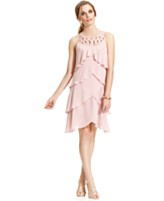
\includegraphics[width=\linewidth]{concepts/concept1_pos1.jpg}
\label{fig:sub1}
\end{subfigure}%
\begin{subfigure}{.18\textwidth}
\centering
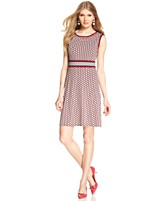
\includegraphics[width=\linewidth]{concepts/concept1_pos2.jpg}
\label{fig:sub2}
\end{subfigure}
\begin{subfigure}{.18\textwidth}
\centering
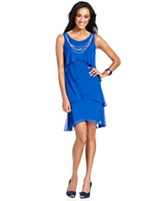
\includegraphics[width=\linewidth]{concepts/concept1_pos3.jpg}
\label{fig:sub2}
\end{subfigure}
\begin{subfigure}{.18\textwidth}
\centering
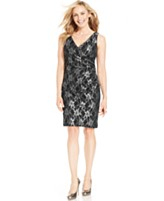
\includegraphics[width=\linewidth]{concepts/concept1_pos4.jpg}
\label{fig:sub2}
\end{subfigure}
\begin{subfigure}{.18\textwidth}
\centering
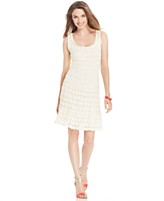
\includegraphics[width=\linewidth]{concepts/concept1_pos5.jpg}
\label{fig:sub2}
\end{subfigure}
\subcaption{The top 5 items, representing the positive direction}

\centering
\begin{subfigure}{.18\textwidth}
\centering
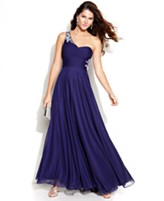
\includegraphics[width=\linewidth]{concepts/concept1_neg1.jpg}
\label{fig:sub1}
\end{subfigure}%
\begin{subfigure}{.18\textwidth}
\centering
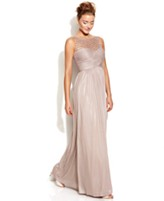
\includegraphics[width=\linewidth]{concepts/concept1_neg2.jpg}
\label{fig:sub2}
\end{subfigure}
\begin{subfigure}{.18\textwidth}
\centering
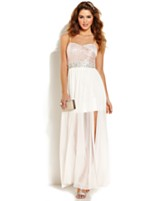
\includegraphics[width=\linewidth]{concepts/concept1_neg3.jpg}
\label{fig:sub2}
\end{subfigure}
\begin{subfigure}{.18\textwidth}
\centering
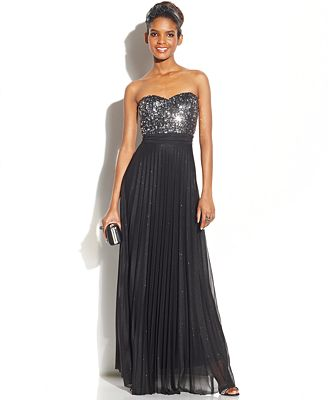
\includegraphics[width=\linewidth]{concepts/concept1_neg4.jpg}
\label{fig:sub2}
\end{subfigure}
\begin{subfigure}{.18\textwidth}
\centering
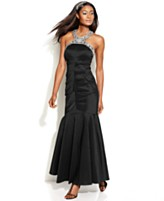
\includegraphics[width=\linewidth]{concepts/concept1_neg5.jpg}
\label{fig:sub2}
\end{subfigure}
\subcaption{The bottom 5 items, representing the negative direction}
\label{fig:conceptA}
\title{Figure 1: The top and bottom items representing a concept in the Dresses
category.  This concept could be characterized as modern and tiered in the
positive direction, and gown-like and elegant in the negative direction.}
\end{figure}

\begin{figure}
\centering
\begin{subfigure}{.18\textwidth}
\centering
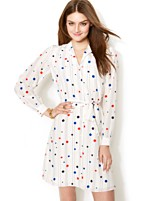
\includegraphics[width=\linewidth]{concepts/concept2_pos1.jpg}
\label{fig:sub1}
\end{subfigure}%
\begin{subfigure}{.18\textwidth}
\centering
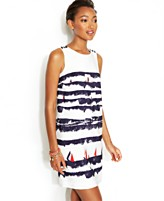
\includegraphics[width=\linewidth]{concepts/concept2_pos2.jpg}
\label{fig:sub2}
\end{subfigure}
\begin{subfigure}{.18\textwidth}
\centering
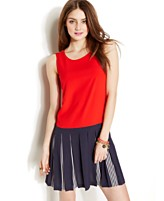
\includegraphics[width=\linewidth]{concepts/concept2_pos3.jpg}
\label{fig:sub2}
\end{subfigure}
\begin{subfigure}{.18\textwidth}
\centering
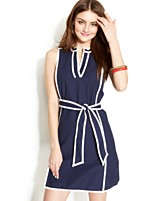
\includegraphics[width=\linewidth]{concepts/concept2_pos4.jpg}
\label{fig:sub2}
\end{subfigure}
\begin{subfigure}{.18\textwidth}
\centering
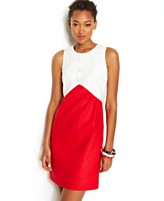
\includegraphics[width=\linewidth]{concepts/concept2_pos5.jpg}
\end{subfigure}
\subcaption{The top 5 items, representing the positive direction}

\centering
\begin{subfigure}{.18\textwidth}
\centering
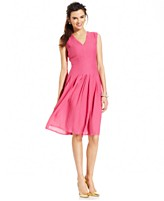
\includegraphics[width=\linewidth]{concepts/concept2_neg1.jpg}
\label{fig:sub1}
\end{subfigure}%
\begin{subfigure}{.18\textwidth}
\centering
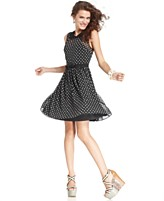
\includegraphics[width=\linewidth]{concepts/concept2_neg2.jpg}
\label{fig:sub2}
\end{subfigure}
\begin{subfigure}{.18\textwidth}
\centering
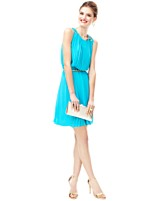
\includegraphics[width=\linewidth]{concepts/concept2_neg3.jpg}
\label{fig:sub2}
\end{subfigure}
\begin{subfigure}{.18\textwidth}
\centering
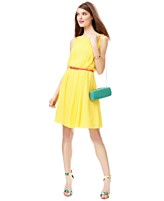
\includegraphics[width=\linewidth]{concepts/concept2_neg4.jpg}
\label{fig:sub2}
\end{subfigure}
\begin{subfigure}{.18\textwidth}
\centering
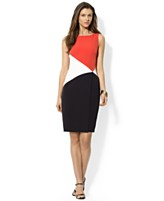
\includegraphics[width=\linewidth]{concepts/concept2_neg5.jpg}
\label{fig:sub2}
\end{subfigure}
\subcaption{The bottom 5 items, representing the negative direction}
\title{Figure 2: The top and bottom items representing another different Dresses
concept. This concept could be characterized as two-toned and playful in the
positive direction, and belted and light in the negative direction.}
\label{fig:conceptB} \end{figure}

\subsubsection*{Concept Space Mapping}
Using random walks to simulate user data, followed by the application of LSI, is
indeed an effective way to encode information from a recommendation graph into a
latent feature space. But what is the relationship between latent feature
vectors derived from disconnected graph partitions? In principle, there is no
guarantee of any relationship between such concept spaces in the same way that
there is no guarantee of any relationship between two arbitrary, disconnected
recommendation graphs. Nonetheless, our hypothesis is that a relationship
between these concept spaces often will exist due to the effectiveness of the
underlying CF techniques that generate the graphs to capture meaningful
item-item associations. Put another way, we believe that the most fundamental
latent dimensions along which products in a category such as Women's swimsuits
vary will be common to many swimsuit catalogues. If this is indeed true, then it
might be possible to learn a mapping between these concept spaces.

If a mapping between the concept spaces associated with two catalogues were
known, we could translate all items into a common space and then choose
inter-catalogue edges between item pairs that are nearest to one another in
concept space. To learn these mapping, we must revisit the notion of content
similarity. Once again, we utilize tf-idf vectors. This time, however, we weight
an item $i$'s tf-idf vector $\vec{\tau}(i)$ by the elements in its latent
feature vector $\vec{v}(i)$. In this way, we construct a dense {\em
super-tf-idf} vector for each concept for each catalogue. Formally, we say that
a concept $j$ of a catalogue $C$ is represented by the super-tf-idf vector
\begin{align}
\vec{s}(j,C) = \sum_{i \in C}{v(i)_j \cdot \vec{\tau}(i)},
\end{align}
where $v(i)_j$ is the $j$\textsuperscript{th} component of item $i$'s latent
feature vector. Note that since the components $v(i)_j$ may be positive or
negative so too can the elements of a concept's super-tf-idf vector, in
constrast to the elements of an individual item's tf-idf vector which are
necessarily greater than or equal to zero. Also note that we compute both
$\vec{s}_1$ and $\vec{s}_2$, which correpond to unigram and bigram super-tf-idf
vectors, respectively, for each concept. These super-tf-idf vectors then act as
proxies for the concept.

With these proxy representations of the concepts for the concept spaces of two
catalogues $C_1$ and $C_2$, we construct a matrix $A$ of inner-products of
super-tf-idf vectors.  Specifically, the matrix elements of $A$ are given by
\begin{align}
A_{ij}(C_1,C_2) = \vec{s}_1(i,C_1) \cdot \vec{s}_1(j,C_2) + \beta \cdot
\vec{s}_2(i,C_1) \cdot \vec{s}_2(j,C_2),
\end{align}
where $i$ is a concept from $C_1$ and $j$ is a concept from $C_2$ and $\beta$ is
the same parameters as before (again, we find $\beta=0.3$ works well).  We may
now use this matrix to transform the vector representation of an item in one
concept space into a vector representation in another concept space.

It is important to note that the transformation matrix $A$ is not orthogonal, and
therefore, does not preserve vector norms. We address this issue by normalizing
all feature vectors, both foreign and domestic, in the concept space following
the transformation. This radially projects all items onto the surface of sphere
within the 16-dimensional concept space. Now when ranking an item's neighbors by
distance, we are actually ranking neighbors by angular separation. That is, we
are ranking neighbors by their cosine similarity in concept space. After
experimenting with various normalization schemes we find that this approach
works best.

Together, these steps comprise the $LatentFeatureRecommender$. First, we
simulate user sessions by randomly walking the recommendation graphs. Second, we
learn concept spaces for products in each catalogue via LSI. Third, we find a
mapping between concept spaces using weighted tf-idf vector representations of
the products. And lastly, we find the nearest neighbors of each product from one
catalogue within the concept space of another catalogue. These nearest neighbors
are then the predicted recommendations between products across the two
catalogues.

\subsubsection*{Popularity}
The $LatentFeatureRecommender$ can be significantly improved by incorporating
the notion of item {\em popularity}. The idea is that a more popular item is
more likely to be recommended, independent of how similar it is. We see signs of
this in the undirected recommendation graphs from www.macys.com. Although each
product has at most four outgoing recommendations on its details page, we see
that some products have over one hundred incoming recommendations. But how
might we define {\em popularity}? A reasonable definition would introduce a
quantity that is correlated with the number of users that indicate a preference
for an item. Like all user data, this is not publicly available information.
Once again, however, we can leverage the recommendation graph to infer an
approximate popularity metric for each item.

We define item popularity as
\begin{align}
\rho(A) = \mathrm{log}(1 + \mathrm{deg}(A)),
\end{align}
where $\mathrm{deg}(A)$ is the degree of the item $A$ within its recommendation
graph.  We find this quanity to be useful in improving the
$LatentFeatureRecommender$ in several ways.

We begin with an attempt to seprate the notion of item similarity from that of
item popularity. The idea that more popular items are more likely to be
recommended than less popular items motivates an alternative mode for conducting
our random walks over a recommendation graph in order to better isolate item
similarity. We do this by adjusting the probability of transitioning to an item
on the graph by making it inversely proportional to that item's popularity,
$\rho$. Stationary distributions learned from these alternative random walks
better reflect item-item similarity. We find that removing item popularity from
our simulated user data results in better success when mapping between the
derived concept spaces (as evidenced by the improved precision and recall
discussed in the next section).

Next, we reincorporate popularity by modifying how we search for nearest
neighbors in concept space. Instead of simply ranking neighbors by distance, we
now rank by distance divided by $\rho$.  In this context, having defined
popularity as the logorithm of node degree reduces the liklihood that one or two
very popular items will always appear as the best recommendations when using
this weighted ranking policy. 

The third way in which popularity is used is determining the number
recommendations alotted per product. We assume that a popular product in one
catalogue is likely to be a popular product in another catalogue. Specifically,
the number of predicted inter-catalogue recommendations predicted per item is
made directly proportional to the item's value of $\rho$.

This assumption is corroborated by the data. The following histogram shows the
number of gold-standard recommendations associated with the top 25 most popular
items, ranked by their value of $\rho$. The histogram also includes the
distribution of predicted recommendations for these items by the
$LatentFeatureRecommender$ both with and without popularity mechanisms. With
popularity, the predictions follow a similar distribution to that of the
gold-standard recommendations. Without popularity, the recommendations are
scattered more uniformly over the thousands of items of each catalogue such that
the number of times these 25 items are recommended is significantly smaller
(barely visible in the plot). This is because the recommendations are based
solely on similarity in concept space (after mapping) and popular items are not
inherently more similar to other items. Importantly, the
$LatentFeatureRecommender$ {\em without popularity} still outperforms the
$ContentBasedRecommender$ demonstrating that while popularity is important, it
is only one of several features that useful in choosing good inter-catalogue
recommendations.

\begin{figure}[!htbp]
    \centering
    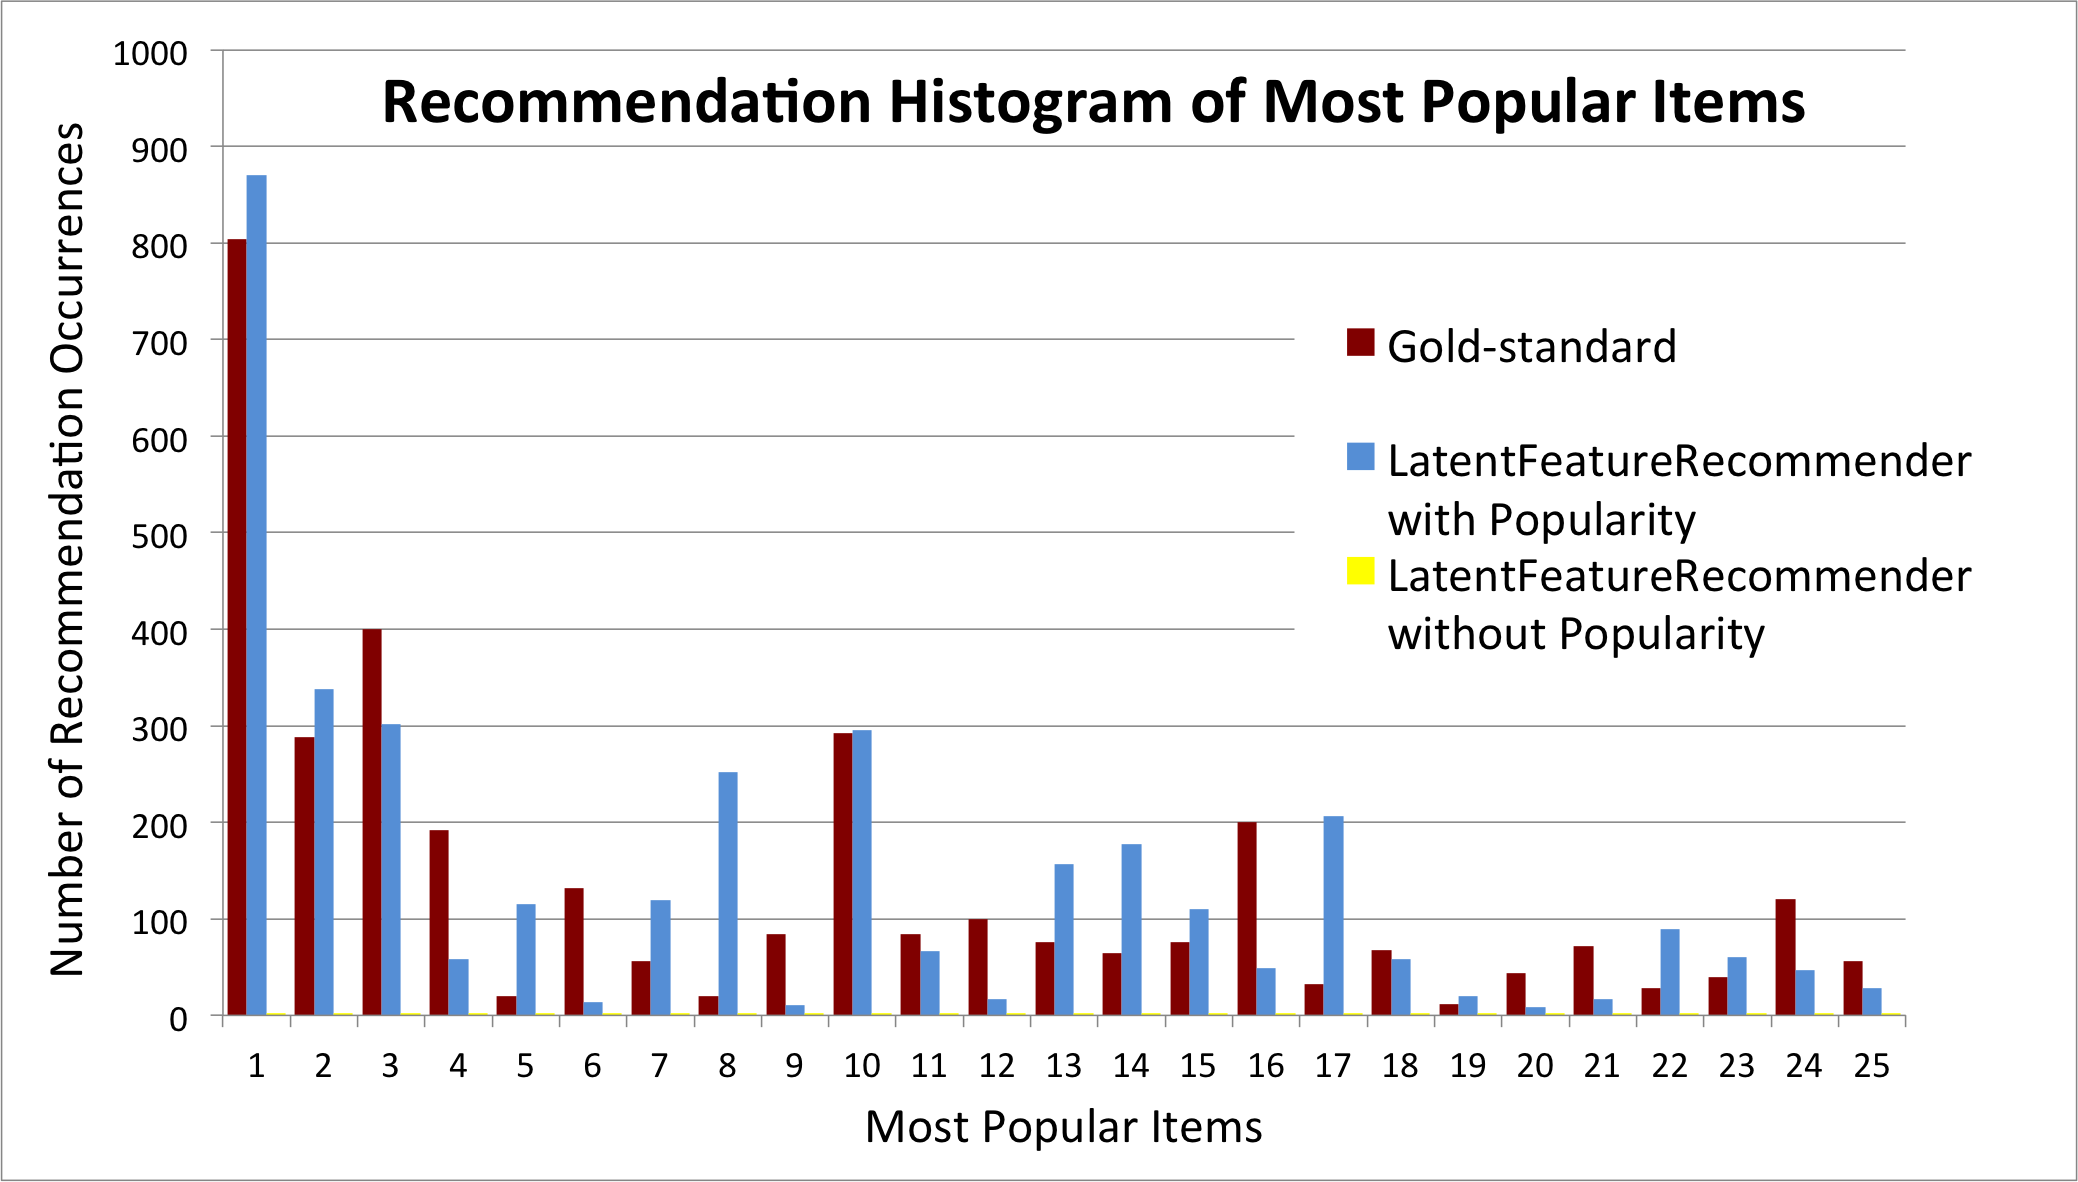
\includegraphics[width=1.0\textwidth]{PopularityHistogram2.png}
	\caption{The top 25 most popular items and how many times they appear in
    recommendations. Here we compare the distribution of gold-standard
    recommendations (red) to the recommendations predicted by the
    $LatentFeatureRecommender$ with (blue) and without (yellow) popularity. The
    yellow bars are small and barely visible. This plot was generated on the
    Women's Dresses category.}
    \label{fig:PopularityHistogram}
\end{figure}

In all, these popularity additions significantly boost the performance of the
\linebreak $LatentFeatureRecommender$. The results of this, along with
comparisons to the other inter-catalogue  recommeder algorithms described in
this section, are provided in the following section.

\section*{Performance}
\subsection*{Baselines}
In addition to the $ContentBasedRecommender$ and the $NeighborhoodRecommender$,
we constructed and tested several other baseline algorithms to compare the
$LatentFeatureRecommender$ against. These baselines show that the performance of
$LatentFeatureRecommender$ is not due to a single mechanism but rather is the
result of the mult-stage algorithm. In this section, we briefly outline these
additional baselines.

\subsubsection*{\em RandomRecommender}
The simplest and least challenging baseline. This recommender randomly chooses a
fixed number of recommendations for each item across catalogues.

\subsubsection*{\em PopularityRecommender}
A baseline that exclusively exploits popularity $\rho$, without any other
knowledge of the recommendation graphs or of item content. This recommender
simply chooses, at random, one of the top three most popular items from the
other catalogue as recommendations for each item in a catalogue. This baseline
aims to demonstrate the efficacy of popularity alone.

\subsubsection*{\em RandomMapRecommender}
This is the $LatentFeatureRecommender$ without the mapping stage. Instead it
generates a random value between -1.0 and 1.0 for each element of the mapping
matrix $A$. As such, it is still leveraging popularity $\rho$ in the same way as
the $LatentFeatureRecommender$. This baseline aims to reveal the importance of
the mapping stage.

\subsubsection*{\em OneModelRecommender}
This is not baseline but rather a cheat. This is the $LatentFeatureRecommender$
except, for this experiment, we defer the graph partitioning until after we have
performed our random walks and constructed a single concept space. Only then do
we partition the items such that their latent feature vectors represent all
items in a single concept space. The goal of this experiment is to determine how
well our algorithm might do if a perfect concept mapping existed and we could
somehow compute it.

\subsection*{Results}

\begin{table}
\begin{center}
\begin{tabular}{ | l || c | c | c || c | c | c |}
\hline
Recommender & Precision & Recall & F1 Score & 2-Precision & 2-Recall & 2-F1 Score \\ \hline\hline
$Random$ & .002 & .001 & .001 & .021 & .008 & .012 \\ \hline
$Popularity$ & .016 & .019 & .017 & .080 & .096 & .087 \\ \hline
$RandomMap$ & .014 & .019 & .016 & .070 & .095 & .081 \\ \hline
$OneModel$ & .103 & .132 & .116 & .404 & .410 & .407 \\ \hline
$ContentBased$ & .014 & .020 & .016 &
\textbf{.115} & \textbf{.186} & \textbf{.142} \\ \hline 
$Neighborhood$ & .040 & .060 & .048 &
\textbf{.137} & \textbf{.240} & \textbf{.175} \\ \hline 
$LatentFeature$ & .036 & .060 & .045 &
\textbf{.174} & \textbf{.228} & \textbf{.197} \\ \hline
\end{tabular}
\caption{The performance of each of the recommenders across all categories. The
first five are the baseline recommenders outlined in the previous section. The
final three are the recommenders of interest, described in the Recommender
Algorithms section. The scores in bold are the most important results and are 
further illustrated in the following figure.}
\end{center}
\end{table}
\begin{figure}[!htbp]
    \centering
    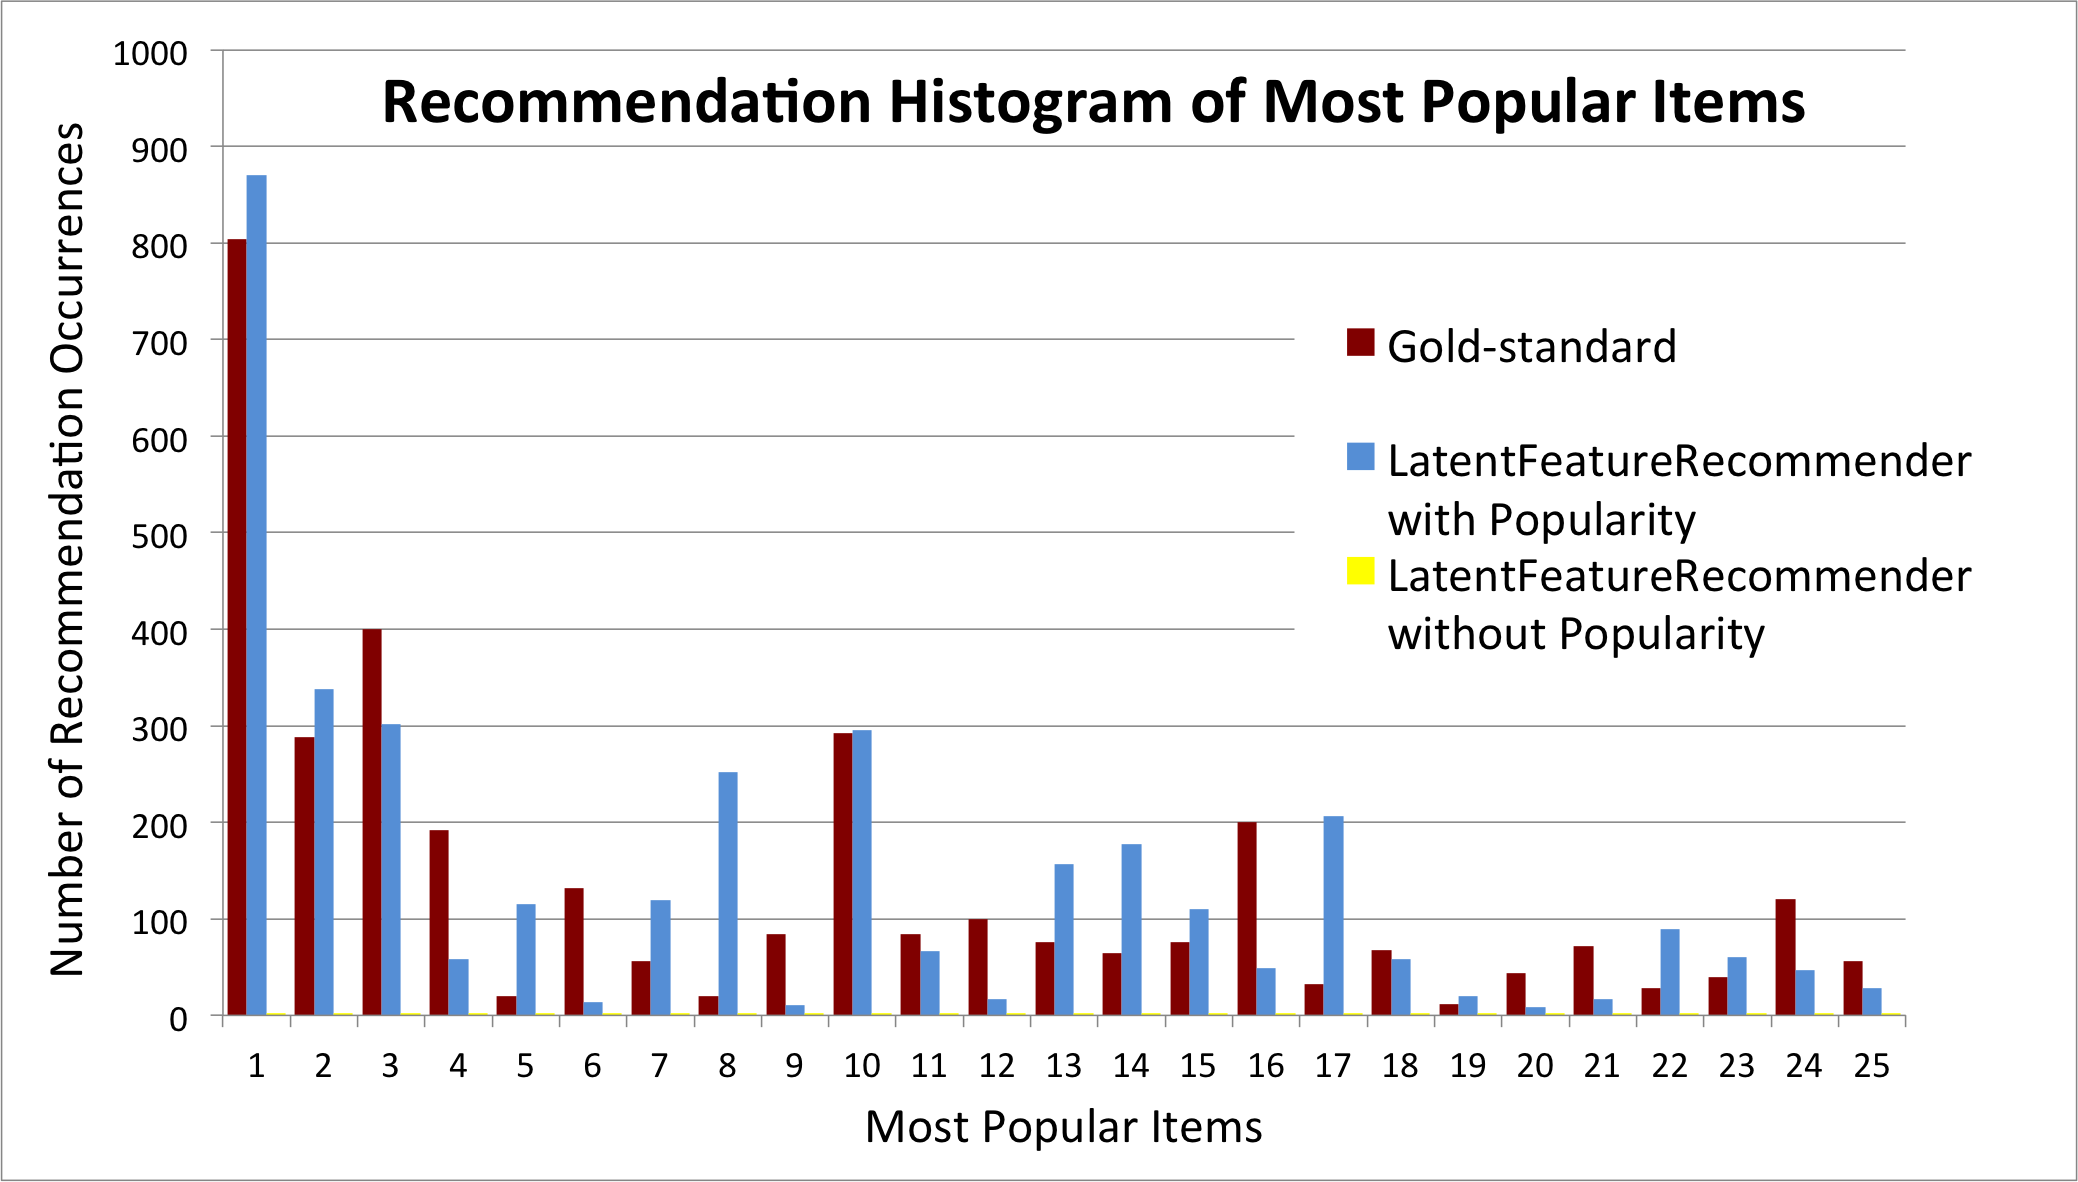
\includegraphics[width=0.75\textwidth]{RecommenderPerformance2.png}
	\caption{The performance of the three main recommenders in terms of
    2-metrics across all categories. We emphasize the 2-F1 Score as our most
    important single metric of comparison. We see that the $LatentFeatureRecommender$
    outperforms the other recommenders in this score.} 
    \label{fig:RecommenderPerformance} 
\end{figure}

Table (1) shows the results of all inter-catalogue recommenders across all
categories. For example, the {\em precision} column lists the sum, across all
categories, of correctly predicted edges divided by the sum, across all
categories, of predicted edges. We first point out that both $Neighborhood$ and
$LatentFeature$ outperform $ContentBased$ by all metrics. This makes clear the
utility of leveraging information from the recommendation when making
inter-catalogue recommendations. Next, we notice that $Neighborhood$ actually
outperforms $LatentFeature$ in {\em precision} by 10\% and in {\em 2-recall} by
about 5\%. Importantly, however, $LatentFeature$ bests $Neighborhood$ in the key
metric {\em 2-}$F_1$ by about 12\%. 


\pagebreak
\section*{Conclusion}
In this study, we address the problem of determining inter-retailer, or
inter-catalogue, item-item associations. We frame this problem as a recommender
problem, which motivates a relatively straightforward experiment in which a
candidate algorithm must connect two recommendation graphs by guessing edges
between them.

In this work, we introduced a novel technique for predicting item-item
associations across retailers. This technique employs {\em Topic-Sensitive
PageRank} on a publicly available recommendation graph to generate simulated
user data. With this data, we perform {\em Latent Semantec Indexing} to learn a
latent feature space for items from in a particular online catalogue. By
generalizing the notion of {\em Term Frequency---Inverse Document Frequency}
score, we construct proxy tf-idf vectors for the latent dimensions, or {\em
concepts}, associated with a particular catalogue. This, in turn, allows us to
construct a transformation matrix such that vectors in one catalogue's concept
space can be transformed into another catalogue's concept space. Inter-catalogue
associations can then be made by finding pairs of items that are a minimal
distance apart in a common concept space.

This technique is improved upon by incorporating the notion of item {\em
popularity} $\rho$, which we define in this context to be the logarithm of the
item's degree within its associated recommendation graph. We show that $\rho$
can be used in multiple ways to improve the performance of an inter-retailer
recommender system.

Finally, we compared our latent inter-catalogue recommender system to several
nontrival baseline algorithms and find that it outperforms all of them in both
standard precision and recall of gold-standard inter-catalogue edges as well as
another combination of informative metrics we call {\em 2-precision} and {\em
2-recall}.

Making accurate item-item associations across retailers using only publicly
available information is a challenging problem. The ability to accurately
identity these relationships, however, could potentially provide a retailer or
other service provider with valuable business intelligence. 

\begin{thebibliography}{9}

\bibitem{Ricci2011}
    Francesco Ricci, Lior Rokach, and Bracha Shapira.
    \emph{Introduction to Recommender Systems Handbook}, Springer, 1-35, 2011.

\bibitem{mgp}
    For information on the Music Genome Project, visit
    http://www.pandora.com/about/mgp

\bibitem{Koren2009}
    Yehuda Koren, Robert Bell, and Chris Volinsky.
    ``Matrix factorization techniques for recommender systems.''
    \emph{Computer} 42.8, 2009. 30-37.

\bibitem{Powers2011}
    David M W Powers.
    ``Evaluation: From Precision, Recall and F-Measure to ROC, Informedness,
Markedness \& Correlation.''
    \emph{Journal of Machine Learning Technologies} \textbf{2}, 37-63, 2011.

\bibitem{Haveliwala2002}
    Taher Haveliwala.
    ``Topic-Sensitive PageRank.''
    \emph{Proceedings of the Eleventh International World Wide Web Conference}
(Honolulu, Hawaii) 2002.

\bibitem{Norris1998}
    James R. Norris.
    \emph{Markov Chains}. Cambridge University Press, 1998.

\bibitem{Deerwester1990}
    Scott Deerwester, Susan T. Dumais, George W. Furnas, Thomas K. Landauer,
Richard Harshman.
    ``Indexing by Latent Semantex Analysis.''
    \emph{American Society for Information Science} \textbf{41}, 391-407, 1990.

\end{thebibliography}

\end{document}
